\documentclass[11pt,a4paper,]{article}
\usepackage{lmodern}

\usepackage{amssymb,amsmath}
\usepackage{ifxetex,ifluatex}
\usepackage{fixltx2e} % provides \textsubscript
\ifnum 0\ifxetex 1\fi\ifluatex 1\fi=0 % if pdftex
  \usepackage[T1]{fontenc}
  \usepackage[utf8]{inputenc}
\else % if luatex or xelatex
  \usepackage{unicode-math}
  \defaultfontfeatures{Ligatures=TeX,Scale=MatchLowercase}
\fi
% use upquote if available, for straight quotes in verbatim environments
\IfFileExists{upquote.sty}{\usepackage{upquote}}{}
% use microtype if available
\IfFileExists{microtype.sty}{%
\usepackage[]{microtype}
\UseMicrotypeSet[protrusion]{basicmath} % disable protrusion for tt fonts
}{}
\PassOptionsToPackage{hyphens}{url} % url is loaded by hyperref
\usepackage[unicode=true]{hyperref}
\hypersetup{
            pdftitle={Understanding Trade},
            pdfborder={0 0 0},
            breaklinks=true}
\urlstyle{same}  % don't use monospace font for urls
\usepackage{geometry}
\geometry{a4paper, centering, text={16cm,24cm}}
\usepackage[style=authoryear-comp,]{biblatex}
\addbibresource{references.bib}
\usepackage{longtable,booktabs}
% Fix footnotes in tables (requires footnote package)
\IfFileExists{footnote.sty}{\usepackage{footnote}\makesavenoteenv{long table}}{}
\IfFileExists{parskip.sty}{%
\usepackage{parskip}
}{% else
\setlength{\parindent}{0pt}
\setlength{\parskip}{6pt plus 2pt minus 1pt}
}
\setlength{\emergencystretch}{3em}  % prevent overfull lines
\providecommand{\tightlist}{%
  \setlength{\itemsep}{0pt}\setlength{\parskip}{0pt}}
\setcounter{secnumdepth}{5}

% set default figure placement to htbp
\makeatletter
\def\fps@figure{htbp}
\makeatother


\title{Understanding Trade}

%% MONASH STUFF

%% CAPTIONS
\RequirePackage{caption}
\DeclareCaptionStyle{italic}[justification=centering]
 {labelfont={bf},textfont={it},labelsep=colon}
\captionsetup[figure]{style=italic,format=hang,singlelinecheck=true}
\captionsetup[table]{style=italic,format=hang,singlelinecheck=true}


%% FONT
\RequirePackage{bera}
\RequirePackage[charter,expert,sfscaled]{mathdesign}
\RequirePackage{fontawesome}

%% HEADERS AND FOOTERS
\RequirePackage{fancyhdr}
\pagestyle{fancy}
\rfoot{\Large\sffamily\raisebox{-0.1cm}{\textbf{\thepage}}}
\makeatletter
\lhead{\textsf{\expandafter{\@title}}}
\makeatother
\rhead{}
\cfoot{}
\setlength{\headheight}{15pt}
\renewcommand{\headrulewidth}{0.4pt}
\renewcommand{\footrulewidth}{0.4pt}
\fancypagestyle{plain}{%
\fancyhf{} % clear all header and footer fields
\fancyfoot[C]{\sffamily\thepage} % except the center
\renewcommand{\headrulewidth}{0pt}
\renewcommand{\footrulewidth}{0pt}}

%% MATHS
\RequirePackage{bm,amsmath}
\allowdisplaybreaks

%% GRAPHICS
\RequirePackage{graphicx}
\setcounter{topnumber}{2}
\setcounter{bottomnumber}{2}
\setcounter{totalnumber}{4}
\renewcommand{\topfraction}{0.85}
\renewcommand{\bottomfraction}{0.85}
\renewcommand{\textfraction}{0.15}
\renewcommand{\floatpagefraction}{0.8}


%\RequirePackage[section]{placeins}

%% SECTION TITLES


%% SECTION TITLES (NEW: Changing sections and subsections color)
\RequirePackage[compact,sf,bf]{titlesec}
\titleformat*{\section}{\Large\sf\bfseries\color[rgb]{0.8, 0.7, 0.1 }}
\titleformat*{\subsection}{\large\sf\bfseries\color[rgb]{0.8, 0.7, 0.1 }}
\titleformat*{\subsubsection}{\sf\bfseries\color[rgb]{0.8, 0.7, 0.1 }}
\titlespacing{\section}{0pt}{2ex}{.5ex}
\titlespacing{\subsection}{0pt}{1.5ex}{0ex}
\titlespacing{\subsubsection}{0pt}{.5ex}{0ex}


%% TITLE PAGE
\def\Date{\number\day}
\def\Month{\ifcase\month\or
 January\or February\or March\or April\or May\or June\or
 July\or August\or September\or October\or November\or December\fi}
\def\Year{\number\year}

%% LINE AND PAGE BREAKING
\sloppy
\clubpenalty = 10000
\widowpenalty = 10000
\brokenpenalty = 10000
\RequirePackage{microtype}

%% PARAGRAPH BREAKS
\setlength{\parskip}{1.4ex}
\setlength{\parindent}{0em}

%% HYPERLINKS
\RequirePackage{xcolor} % Needed for links
\definecolor{darkblue}{rgb}{0,0,.6}
\RequirePackage{url}

\makeatletter
\@ifpackageloaded{hyperref}{}{\RequirePackage{hyperref}}
\makeatother
\hypersetup{
     citecolor=0 0 0,
     breaklinks=true,
     bookmarksopen=true,
     bookmarksnumbered=true,
     linkcolor=darkblue,
     urlcolor=blue,
     citecolor=darkblue,
     colorlinks=true}

\usepackage[showonlyrefs]{mathtools}
\usepackage[no-weekday]{eukdate}

%% BIBLIOGRAPHY

\makeatletter
\@ifpackageloaded{biblatex}{}{\usepackage[style=authoryear-comp, backend=biber, natbib=true]{biblatex}}
\makeatother
\ExecuteBibliographyOptions{bibencoding=utf8,minnames=1,maxnames=3, maxbibnames=99,dashed=false,terseinits=true,giveninits=true,uniquename=false,uniquelist=false,doi=false, isbn=false,url=true,sortcites=false}

\DeclareFieldFormat{url}{\texttt{\url{#1}}}
\DeclareFieldFormat[article]{pages}{#1}
\DeclareFieldFormat[inproceedings]{pages}{\lowercase{pp.}#1}
\DeclareFieldFormat[incollection]{pages}{\lowercase{pp.}#1}
\DeclareFieldFormat[article]{volume}{\mkbibbold{#1}}
\DeclareFieldFormat[article]{number}{\mkbibparens{#1}}
\DeclareFieldFormat[article]{title}{\MakeCapital{#1}}
\DeclareFieldFormat[article]{url}{}
%\DeclareFieldFormat[book]{url}{}
%\DeclareFieldFormat[inbook]{url}{}
%\DeclareFieldFormat[incollection]{url}{}
%\DeclareFieldFormat[inproceedings]{url}{}
\DeclareFieldFormat[inproceedings]{title}{#1}
\DeclareFieldFormat{shorthandwidth}{#1}
%\DeclareFieldFormat{extrayear}{}
% No dot before number of articles
\usepackage{xpatch}
\xpatchbibmacro{volume+number+eid}{\setunit*{\adddot}}{}{}{}
% Remove In: for an article.
\renewbibmacro{in:}{%
  \ifentrytype{article}{}{%
  \printtext{\bibstring{in}\intitlepunct}}}

\AtEveryBibitem{\clearfield{month}}
\AtEveryCitekey{\clearfield{month}}

\makeatletter
\DeclareDelimFormat[cbx@textcite]{nameyeardelim}{\addspace}
\makeatother

\author{\sf\Large\textbf{ Prachi Jaiswal}\\ {\sf\large Undergraduate\\[0.5cm]} \sf\Large\textbf{ Yuwei Jiang}\\ {\sf\large Master\\[0.5cm]} \sf\Large\textbf{ Sithalakshmi Jawahar}\\ {\sf\large Undergraduate\\[0.5cm]}}

\date{\sf\Date~\Month~\Year}
\makeatletter
\lfoot{\sf Jaiswal, Jiang, Jawahar: \@date}
\makeatother


%%%% PAGE STYLE FOR FRONT PAGE OF REPORTS

\makeatletter
\def\organization#1{\gdef\@organization{#1}}
\def\telephone#1{\gdef\@telephone{#1}}
\def\email#1{\gdef\@email{#1}}
\makeatother
  \organization{ETC5513 Assignment4 Team Nemo}

  \def\name{Monash University \newline Business and Economics}

  \telephone{(03) 9905 2478}

  \email{questions@company.com}                 %NEW: New email addresss

\def\webaddress{\url{http://company.com/stats/consulting/}} %NEW: URl
\def\abn{12 377 614 630}                                    % NEW: ABN
\def\logo{\includegraphics[width=6cm]{Figures/logo}}  %NEW: Changing logo
\def\extraspace{\vspace*{1.6cm}}
\makeatletter
\def\contactdetails{\faicon{phone} & \@telephone \\
                    \faicon{envelope} & \@email}
\makeatother

%%%% FRONT PAGE OF REPORTS

\def\reporttype{Report for}

\long\def\front#1#2#3{
\newpage
\begin{singlespacing}
\thispagestyle{empty}
\vspace*{-1.4cm}
\hspace*{-1.4cm}
\hbox to 16cm{
  \hbox to 6.5cm{\vbox to 14cm{\vbox to 25cm{
    \logo
    \vfill
    \parbox{6.3cm}{\raggedright
      \sf\color[rgb]{0.8, 0.7, 0.1 }    % NEW color 
      {\large\textbf{\name}}\par
      \vspace{.7cm}
      \tabcolsep=0.12cm\sf\small
      \begin{tabular}{@{}ll@{}}\contactdetails
      \end{tabular}
      \vspace*{0.3cm}\par
      ABN: \abn\par
    }
  }\vss}\hss}
  \hspace*{0.2cm}
  \hbox to 1cm{\vbox to 14cm{\rule{4pt}{26.8cm}\vss}\hss\hfill}  %NEW: Thicker line
  \hbox to 10cm{\vbox to 14cm{\vbox to 25cm{   
      \vspace*{3cm}\sf\raggedright
      \parbox{11cm}{\sf\raggedright\baselineskip=1.2cm
         \fontsize{24.88}{30}\color[rgb]{0, 0.29, 0.55}\sf\textbf{#1}}   % NEW: title color blue
      \par
      \vfill
      \large
      \vbox{\parskip=0.8cm #2}\par
      \vspace*{2cm}\par
      \reporttype\\[0.3cm]
      \hbox{#3}%\\[2cm]\
      \vspace*{1cm}
      {\large\sf\textbf{\Date~\Month~\Year}}
   }\vss}
  }}
\end{singlespacing}
\newpage
}

\makeatletter
\def\titlepage{\front{\expandafter{\@title}}{\@author}{\@organization}}
\makeatother

\usepackage{setspace}
\setstretch{1.5}

%% Any special functions or other packages can be loaded here.
\usepackage{booktabs}
\usepackage{longtable}
\usepackage{array}
\usepackage{multirow}
\usepackage{wrapfig}
\usepackage{float}
\usepackage{colortbl}
\usepackage{pdflscape}
\usepackage{tabu}
\usepackage{threeparttable}
\usepackage{threeparttablex}
\usepackage[normalem]{ulem}
\usepackage{makecell}
\usepackage{xcolor}


\begin{document}
\titlepage

\section*{Introduction}

\section*{Germany}

Germany is the most powerful economy of Europe with the biggest export commodities as automobiles and medicament. Besides, we all are aware of the fact that Germany exports a large number of automobiles and their parts to different countries. But did you know that for Germany, the import of automobiles also plays an important role in its trade markets? This can be seen through the below graph:

\begin{figure}[H]
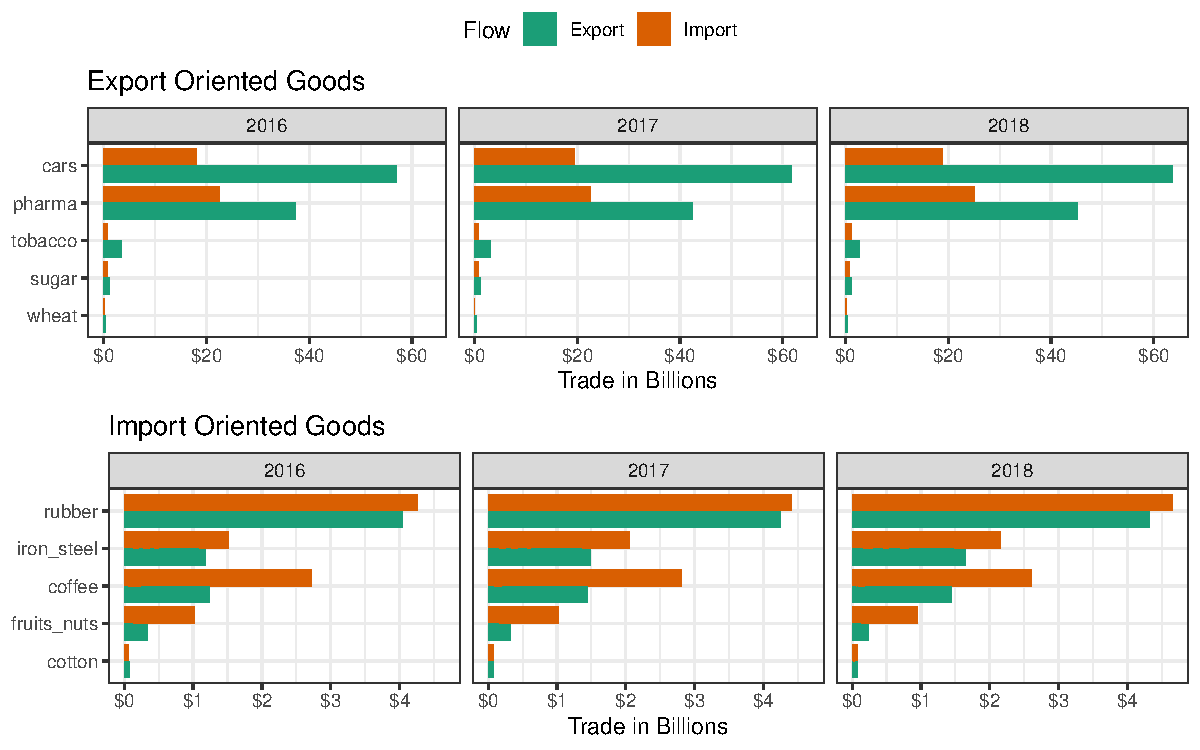
\includegraphics[width=1\linewidth,]{report_files/figure-latex/gtrade-1} \caption{Traded Goods in Germany}\label{fig:gtrade}
\end{figure}

The first section of figure \ref{fig:gtrade} shows the Export-oriented trading goods of Germany where one can see that the Automobiles sector indeed has more Export value than any other sector taken into consideration followed by Pharmaceuticals and Tobacco goods. The export values of these commodities have seen quite a significant rise in their export values. Besides this, Wheat had a slightly negligible import in the year 2016, however, its value saw an increase over the period.

Talking about import, the next section of the same figure (figure \ref{fig:gtrade}) displays a brief insight on the Import oriented trading commodities in Germany. Rubber out-stands every import dominant goods are taken into the study with almost about similar export value. Similarly, for iron and steel, we notice a minor difference in their trade values. Next in the line is Coffee with the 2nd highest Import value and sort of remains parallel over the span. Fruits \& Nuts and Coffee are atypical commodity with their Import value soaring much higher than their Exports.

\begin{table}[!h]

\caption{\label{tab:germanytrend}Trend of Trade in Germany in USD for 3 years}
\centering
\begin{tabular}[t]{r|r}
\hline
Year & Mean\_Trade\\
\hline
2016 & 740559766\\
\hline
2017 & 826727733\\
\hline
2018 & 884902006\\
\hline
\end{tabular}
\end{table}

Table \ref{tab:germanytrend} shows the mean value by Year of all the commodities traded in Germany. The table displays that the Trade value (Export value and Import Value) for 2016 is about 700 million USD. This increases by about 100 million more in the year 2017. And for 2018, it is nearly about 900 million USD. Hence the trade over these years has seen quite a bit increase.

\begin{table}[!h]

\caption{\label{tab:germanycomo}Traded Comodities in Germany}
\centering
\begin{tabular}[t]{l|r|r|r}
\hline
Category & Ex\_Value & Im\_Value & Trend\\
\hline
\cellcolor{gray!6}{cars} & \cellcolor{gray!6}{3556599614} & \cellcolor{gray!6}{1659647794} & \cellcolor{gray!6}{1896951819.6}\\
\hline
pharma & 3096824046 & 2003959050 & 1092864996.5\\
\hline
\cellcolor{gray!6}{tobacco} & \cellcolor{gray!6}{502254364} & \cellcolor{gray!6}{271617658} & \cellcolor{gray!6}{230636705.9}\\
\hline
sugar & 161617581 & 113668563 & 47949018.2\\
\hline
\cellcolor{gray!6}{wheat} & \cellcolor{gray!6}{61969300} & \cellcolor{gray!6}{22357247} & \cellcolor{gray!6}{39612053.3}\\
\hline
rubber & 262819437 & 233275457 & 29543979.4\\
\hline
\cellcolor{gray!6}{cotton} & \cellcolor{gray!6}{7928467} & \cellcolor{gray!6}{8088379} & \cellcolor{gray!6}{-159911.7}\\
\hline
iron\_steel & 166290334 & 175106568 & -8816233.8\\
\hline
\cellcolor{gray!6}{coffee} & \cellcolor{gray!6}{112882680} & \cellcolor{gray!6}{153919437} & \cellcolor{gray!6}{-41036756.6}\\
\hline
fruits\_nuts & 42061094 & 215603589 & -173542495.7\\
\hline
\end{tabular}
\end{table}

From table \ref{tab:germanycomo} can be observed, net trading can be observed in the table. Where there are more exports (positive values) than Imports (negative values) making this a largely export-oriented country. Automobiles and Medicament contributing the most while Coffee and Iron \& Steel contributing very less. Fruits and Nuts rank the lowest as it's imported in much higher value than what it is being exported.
From the table, cars are exported at the highest rate of 1.89 Billion and cotton is imported the most.

\section*{China}

\hypertarget{the-trades-of-china}{%
\section{The trades of China}\label{the-trades-of-china}}

It is reported from Wikipedia(2020) that China has become the world's largest economy by GDP. Due to the rapid growth of China's economy, Chinese trade has expanded at a breakneck pace. This section will concentrate on the analysis of China's performance on world's major varieties of trade.

\hypertarget{import-trades-of-china-from-2016-to-2018}{%
\subsection{Import Trades of China from 2016 to 2018}\label{import-trades-of-china-from-2016-to-2018}}

\begin{figure}[H]
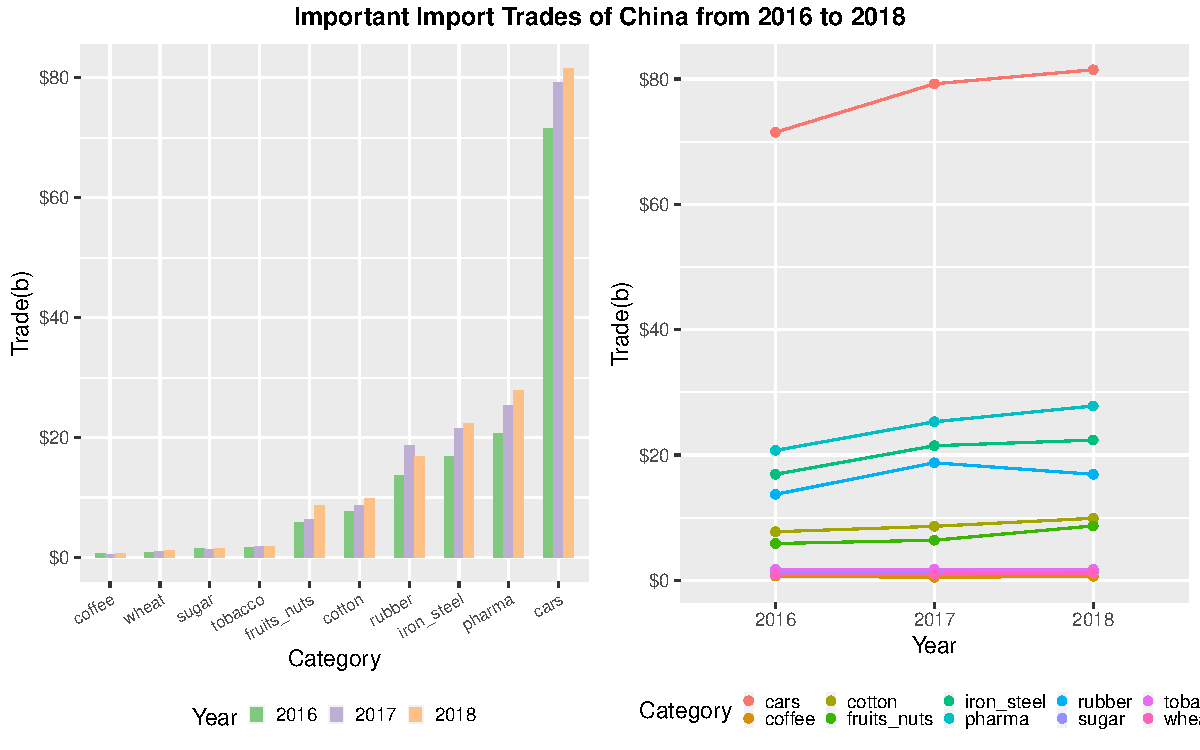
\includegraphics[width=1\linewidth,]{report_files/figure-latex/Yuweiplot1-1} \caption{Important Import Trade of China From 2016 to 2018}\label{fig:Yuweiplot1}
\end{figure}

From the Figure \ref{fig:Yuweiplot1}, it could be concluded that cars, pharma, iron\_steel and rubber are the top four categories that China imported from 2016 to 2018. At the same time, coffee, wheat, sugar and tobacco are not so prosperous among China's import trades. It is worth noting that the total volumes of cars' trades in each year are much higher than that of the second place. When look at the right part of the Figure \ref{fig:Yuweiplot1}, the trade tendencies of the most categories are going smoothly or upward, except for rubber.

\hypertarget{export-trades-of-china-from-2016-to-2018}{%
\subsection{Export trades of China from 2016 to 2018}\label{export-trades-of-china-from-2016-to-2018}}

\begin{figure}[H]
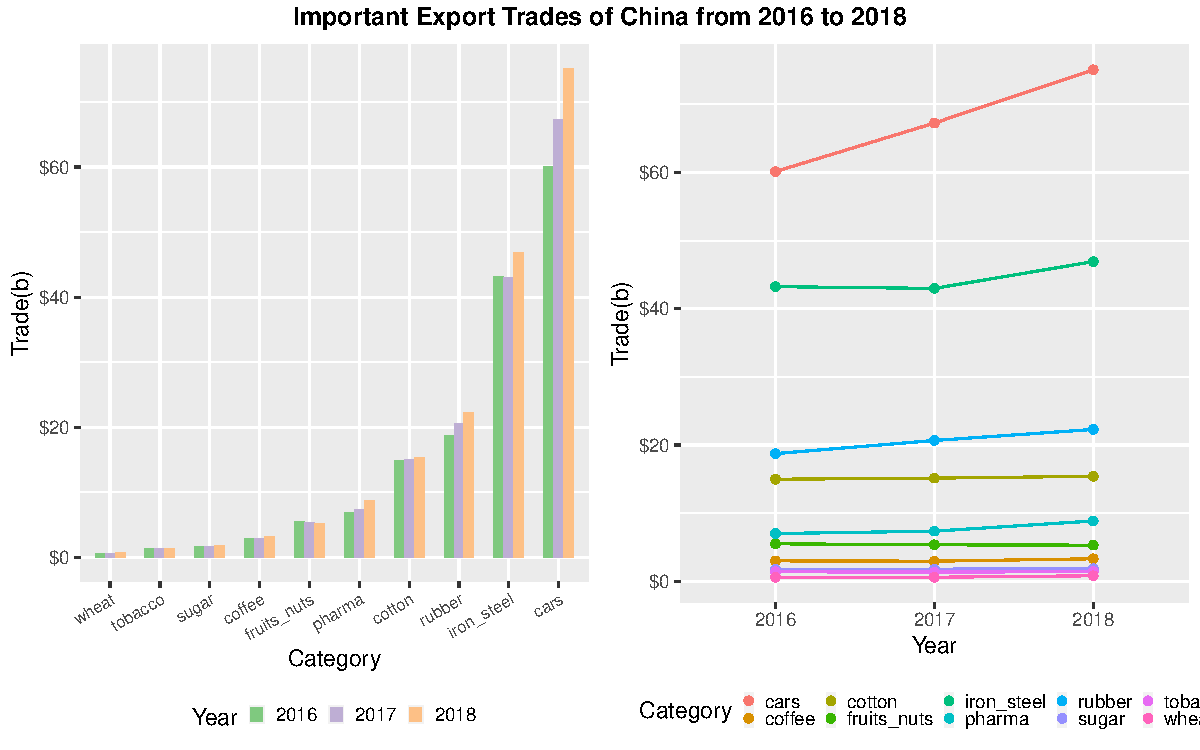
\includegraphics[width=1\linewidth,]{report_files/figure-latex/Yuweiplot2-1} \caption{ Important Export Trade of China From 2016 to 2018}\label{fig:Yuweiplot2}
\end{figure}

Figure \ref{fig:Yuweiplot2} shows the important export trades of China from 2016 to 2018. It could be seen that cars, iron\_steel, rubber and cotton are the top four categories that China exported from 2016 to 2018. At the same time, wheat, tobacco, sugar and coffee are not that popular among China's export trades. It is interesting to see cars, iron\_steel and rubber are also appear in the top four of export trade. And cotton took pharma's place in the export trades. The right part of the Figure \ref{fig:Yuweiplot2} demonstrates that the total volumes of all the ten categories in 2018 are higher than that of 2016 more or less.

\hypertarget{balance-of-trade}{%
\subsection{Balance of trade}\label{balance-of-trade}}

\begin{figure}[H]
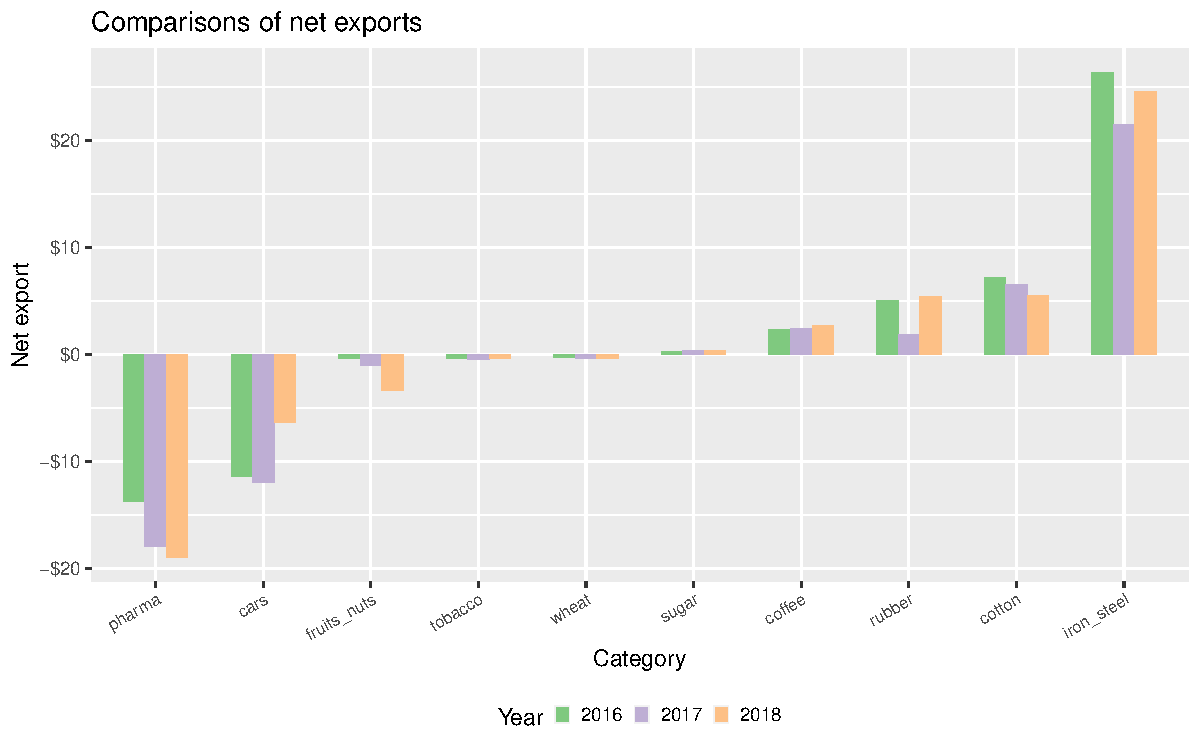
\includegraphics[width=1\linewidth,]{report_files/figure-latex/Yuweiplot3-1} \caption{Comparisons of net exports}\label{fig:Yuweiplot3}
\end{figure}

When we compare the total trades between import and export trades of China, we could draw some conclusions:\\
1.Though the trades of iron\_steel win a place in the top4 both in import and export trades of China,the export trades of iron\_steel are much larger than that of import trades. Imports are less than half of exports.\\
2. Though the import trades of cars are higher than export trades these years, there is a good upward momentum in the tendency of export trades of cars. It might be predicted that the export trades of cars will be more than import cars trades sooner or later.\\
3. The status of imported pharma trades are higher than that of export trades. And from 2016 to 2018 the amount of imports is getting higher year after year. It might be implied that China is somewhat dependent on imported medicine or medical instruments.

\section*{United States of America}

\hypertarget{understanding-the-trend}{%
\subsection{Understanding the trend}\label{understanding-the-trend}}

\begin{figure}[H]
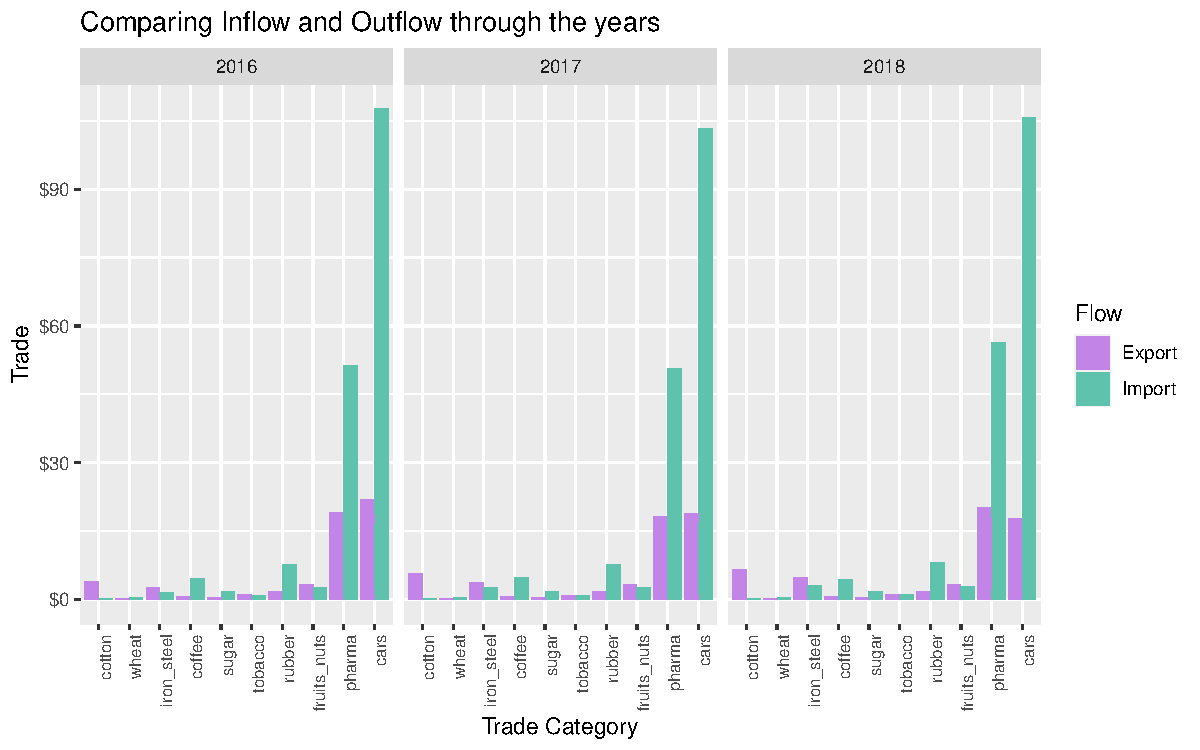
\includegraphics[width=1\linewidth,]{report_files/figure-latex/plot1-1} \caption{Flow of goods}\label{fig:plot1}
\end{figure}

From \ref{fig:plot1} It is obvious that cars are the most traded goods. Even though USA has its own In-house production unit for car brands like Jeep, Ford and Chevrolet it still seems to import a lot of cars at a value of almost 100 billion. Followed by Pharmaceutical products and rubber contributing highly.

Even though USA imports more than it exports, goods like Cotton, fruits and nuts, iron and steel the exports are higher than imports.

\hypertarget{net-trade}{%
\subsection{Net Trade}\label{net-trade}}

\begin{figure}[H]
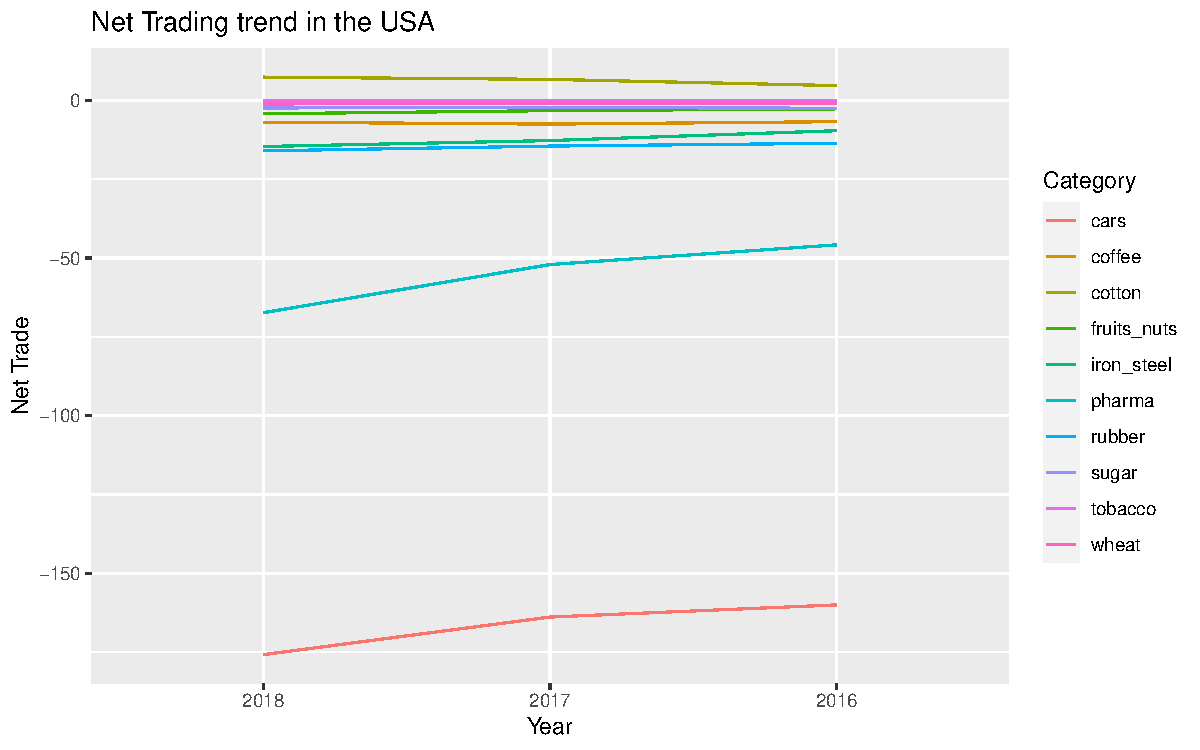
\includegraphics[width=1\linewidth,]{report_files/figure-latex/plot2-1} \caption{Net trading trend}\label{fig:plot2}
\end{figure}

From \ref{fig:plot2} it has become obvious that USA is a more Import oriented economy than an export oriented one because a majority of the lines lie below 0 indicating that it is import. Even here it can be observed that cotton is exported more than it is imported all with an upward trend. Cars and Iron and steel seem to have a downward trend. The most interesting observation is that wheat is imported exactly as much as it is imported. While all the other products are seeing an upward trend and almost exported as much as they are imported.

\section*{Conclusion}

\printbibliography

\end{document}

